\chapter{Introduction}
\section{Background}
% \label{chap:introduction}
Environmental pollution has long been the subject of discussion in the energy and transportation industry, both among policy makers, industry professionals and researchers alike. The continued use of fossil fuels over the decades, in the form of coal, oil and natural gas for a plethora of applications such as power generation, transportation, industrial and large scale manufacturing processes has seen the gradual deterioration of air quality and life \cite{EnergyInformationAdministration2018U.S.2017}.

In recent times, especially in the power generation sector, the use of generative gas turbines for electricity has been preferred over nuclear fuel due to the dire consequences nuclear energy possesses. Nonetheless, the use of gas turbines has not been without its setbacks; its harmful effects particularly, as relates to pollution and emissions from heavy duty fuels, in the form of \ce{SO2}, \ce{NO} and gaseous hydrocarbons \cite{Timko2010ParticulateFuel}. As a result of the policy to curb carbon emissions in and greenhouse gases (GHG), there has been increasing attention to the research of reducing carbon emissions in jet fuels for aero-derivative gas turbine engines \cite{Timko2010ParticulateFuel}. While traditional fossil fuels account for 81\% of US energy demands, it is expected to fall in the near future with the rise of new renewable technologies \cite{EnergyInformationAdministration2018U.S.2017}. 

\begin{figure}[ht]
    \centering
    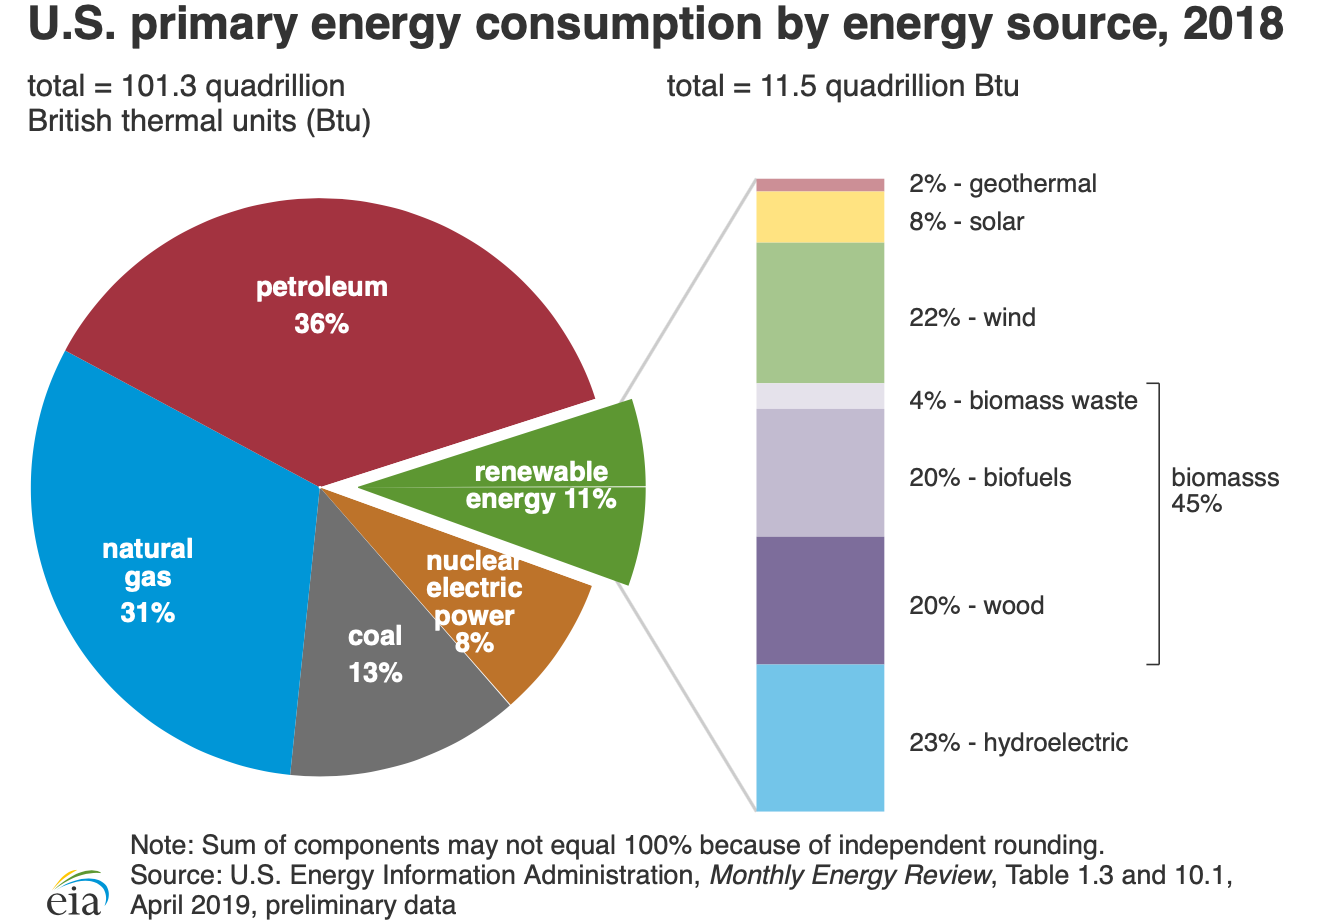
\includegraphics[width=\textwidth, height=\textheight, keepaspectratio]{images/chart-2.png}
    \caption{U.S. primary energy consumption by energy source, 2018 \cite{EnergyInformationAdministration2019Monthly2019}}
    \label{fig:energy demand}
\end{figure}


Notwithstanding, the reliance of power generation on fossil fuels particularly in the heavy duty and aviation industry is without a match at the moment and for some time to come \cite{NationalsAcademiesofSciences2016CommercialResearch}. In lieu of these facts, it is pertinent to abound and comply with emission and pollution regulations designed to curb harmful byproducts of fossil fuels for power generation and transportation by the research, modeling and adoption of alternative non-petroleum based fuels. 

The transportation industry, especially air transport, has long been powered by traditional fossil fuels commonly known as jet fuel. Jet fuels typically consist of carbon-carbon bonded chains blended together with other mixtures. The traditional jet fuels used in commercial air transport typically consist of Jet-A1,JP-8 and JP-10 \cite{NationalsAcademiesofSciences2016CommercialResearch}. These traditional jet fuels however, consist of harmful blends that have the tendency to increase emissions levels and go beyond the limits set by the regulatory environmental agencies. Most of these traditional fuels consist of aromatics that induce particulate matter as well as other volatile organic compounds in the environment and can decrease the life cycle of jet engines based on the refining processes employed \cite{Corporan2007EmissionsFuel}. As a result, efforts have been made to introduce alternative jet fuel blends such as Fischer-Tropsch (F-T) fuels in commercial and military aviation. 

The alternative jet fuels are being synthesised based on mass spectrometry and chromatography analyses to observe the composition of the main driver species behind the high emissions level. The alternative fuels already being used are economical in the sense that, they do not require the extra cost of re-designing existing engines but can be retrofitted to serve as drop in fuels to existing engines \cite{NationalsAcademiesofSciences2016CommercialResearch}. 

\section{Motivation}
Traditional jet fuels typically have \ce{NOx}, \ce{SOx} and particulate matter, but with improved catalytic and synthesis processes, these fuels can be derived from lower carbon fules such as methane or synthesised processes, free of sulphur, nitrogen and contain very little to no aromatics that cause soot \cite{Boogaard2017ToxicologicalToxicology}. There are existing alternative transportation fuels that promise reduced emission such as Liquefied Natural Gas (LNG) fuels, oxygenated fuels such as dimethylether (DME) and other sustainable alternative jet fuels. These alternative jet fuels are being derived through various synthesis and catalytic processes to produce fuels that promise reduced emissions and carbon concentration to the environment\cite{Whale2018ToxicologicalEcotoxicology}. The sustainable aspect refers to the push for fuels that reduce pollution and emissions with a goal of having little to no pollutants, while alternative refers to the method and processes used to refine the fuel - non-petroleum based processes \cite{NationalsAcademiesofSciences2016CommercialResearch}. 

One of the commonly used alternative jet fuels already being used in circulation is the Gas-to-Liquid alternative jet fuel. They are derived from natural gas as feedstock and synthesised through the Fischer-Tropsch (F-T) \cite{Speight2014ChapterProcess} Process in the presence of catalysts to remove unwanted mixtures such as \ce{CO} in the fuels. GTL fuels promise lower \ce{CO2} emissions and can still be used in existing engines without the need to redesign the engines \cite{Corporan2007EmissionsFuel}. Most importantly, these alternative jet fuels (GTL fuels) comply with the existing regulations for emissions and pollution limits for jet fuels as they are already being used both as primary jet fuels and being blended with other compounds to achieve the desired regulatory limits for jet fuel emissions. 
\cleardoublepage
\section{Fischer- Tropsch Gas-to-Liquid (GTL) Fuels}
Gas-to-Liquids (GTL) are essentially catalytic processes that take existing natural gases through either a Methanol synthesis or Fischer-Tropsch (F-T) synthesis. This work is focused on the recovery of GTL through the F-T synthesis to obtain longer carbon chain with high energy content such as gasoline, jet fuel and diesel fuels in the carbon-carbon bonds \cite{U.S.EIA}. The chemistry of the F-T process is a catalytic chemical reaction that was developed in Mülheim an der Ruhr, Germany at the Kaiser Wilhelm Institut für Kohlenforschung by Franz Fischer and Hans Tropsch. This process was named after the inventors and is known as the ‘Fischer–Tropsch process’ \cite{Boogaard2017ToxicologicalToxicology}.
It involves the reaction of carbon monoxide \ce{CO} and hydrogen \ce{H2} in syngas conversion to hydrocarbons of various molecular weights. Controlled by the chemical equation:

  \reaction{(2n + 1) H2 + nCO \longrightarrow C_n H_{2n+2} + nH2O }

Where $n$ is an integer, and when $n$=1, it indicates methane being formed, which is often thought to be an unfavorable byproduct. This reaction also produces significant byproducts such as the water-gas-shift reaction. 
\reaction{CO + H2O \longrightarrow H2 + CO2 }

\begin{figure}[ht]
    \centering
    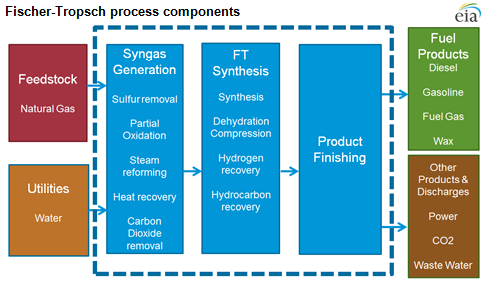
\includegraphics{images/chart2.png}
    \caption{Fischer-Tropsch Synthesis \cite{Mallik2014Gas-to_liquidsMarket}}
    \label{fig:F-T synthesis}
\end{figure}
The conditions typically chosen for the F-T synthesis is made such that there is formation of large hydrocarbons in the presence of catalysts such as Nickel \ce{Ni},Iron\ce{Fe},Cobalt\ce{Co} and Ruthenium \ce{Ru}. While Nickel tends to favor the formation of methane \ce{CH4}, Iron is more economical and also guarantees a higher water-gas-shift activity, it is more suitable when there is low hydrogen/carbon monoxide ration in the syngas such as that in coal gasification \cite{Schulz1999ShortSynthesis}. This process is typically referred to as Reforming \cite{Boogaard2017ToxicologicalToxicology}. This reforming process eliminates harmful vapors that are can cause damage to engines and the environment when combustion occurs. 


These GTL fuels can also serve as alternatives to traditional diesel fuels and heavy carbon fuels, like fuel oils used in heavy machinery based on the low emissions and pollution levels \cite{Timko2010ParticulateFuel}. Since these GTL fuels are going to be used in existing engines. It is imperative to understand the physical and chemical properties of these fuels under engine-like conditions to order to continue the adoption of these fuels as sustainable alternative replacements to traditional jet fuels derived from petroleum-based processes. Furthermore, since engine designers need fuel models as close to the real physical fuel as possible, in order to make real-life simulations of fuel reactivity under engine-like condition, methods like computational fluid dynamic (CFD) model engines are employed to predict the thermal stresses, deformation, fatigue and transport characteristics of these fuel. Thus, it is imperative to look at the possibility of researching fuel models known as chemical kinetic mechanisms that closely represents the real fuel under engine-like conditions as well as the elementary reaction pathways that occur when such fuels are used.


\section{Surrogate Models}
\subsection{What are Surrogate Models ?}
Surrogate models are easily interpretable models of complex physical systems typically used in engineering applications where direct analysis of a system, variables or outcome cannot be measured explicitly \cite{molnar2019}. 
Over the course of the last few decades, surrogate modeling in the form of numerical approximations has become more computationally expensive as the technological advances in computing improves, due to the more demand on making more numerical models that closely match physical systems. This has made engineering tasks more demanding and longer to complete as more fields in system optimization employ these techniques. These surrogate models are often used to significantly reduce both the computational cost and time for numerical approximations. Surrogate models employ the unique technique of evaluating an original function or model at approximate points based on mathematical or physical deductions of the system behavior. Since surrogate modeling is at the heart of numerical optimization, it is often used as a means to deduce what consists of a complex physical system as well as its behavior. Within surrogate modeling optimization, derivatives are often imposed, since optimization usually requires gradient-based algorithms for efficacy and approximate solutions \cite{Bouhlel2019ADerivatives}. These derivatives in the context of chemical systems, require the use of mass spectrometry to determine what constitutes a complex system.

\subsection{Why Surrogate Models ?}
Engine designers of heavy duty machinery especially gas turbines, generally develop new designs of gas turbines through the use of computational models\cite{Mehl2012ModelingApproach}. These computational models involve the use of mathematical representations of physical systems. For engines, as a result of the mechanism for power generation in internal combustion engines (IC), designers and engineers use multi-physics based models of fluid flow to integrate both mass, heat and chemical kinetic models together for a holistic and robust approximation of the physical system through the implementation of computational fluid dynamic (CFD) calculations. These models are usually performed in order to optimize and characterise emission and pollution levels. In order to do this for IC engines, it is pertinent to include the complex chemical reaction pathways involved in the realization of these models. 

\subsection{Surrogate modeling in chemical kinetic mechanisms of fuels}
Chemical reactions of transportation fuels involve large chemical compounds consisting of hundreds and thousands of chemical species, which would prove to be physically impossible to model individually. As such a lumped representation of the large complex chemical compounds can be used to model what is the resulting overall fuel compound. This method of using a lumped representation of complex physical and chemical systems is known as surrogate modeling. 

GTL fuels are blended fuels with a combination of varieties of other pure primary reference fuel compounds based on spectrometry analyses. In order to represent this blended fuel model it is important to know the primary composition of this fuel. Many alternative jet fuels have been used in recent times such as the F-T derived and biomass derived alternative jet fuel surrogate blends of n-alkanes and iso-alkanes in Naik et al\cite{Naik2011DetailedFuels} as well as those used in the work of Dagaut et al for surrogate blends of n-alkane,iso-alkane and alkyl-cycloalkanes in \cite{Dagaut2014} to represent the main composition of a real F-T GTL fuel. 

\begin{figure}[ht]
    \centering
    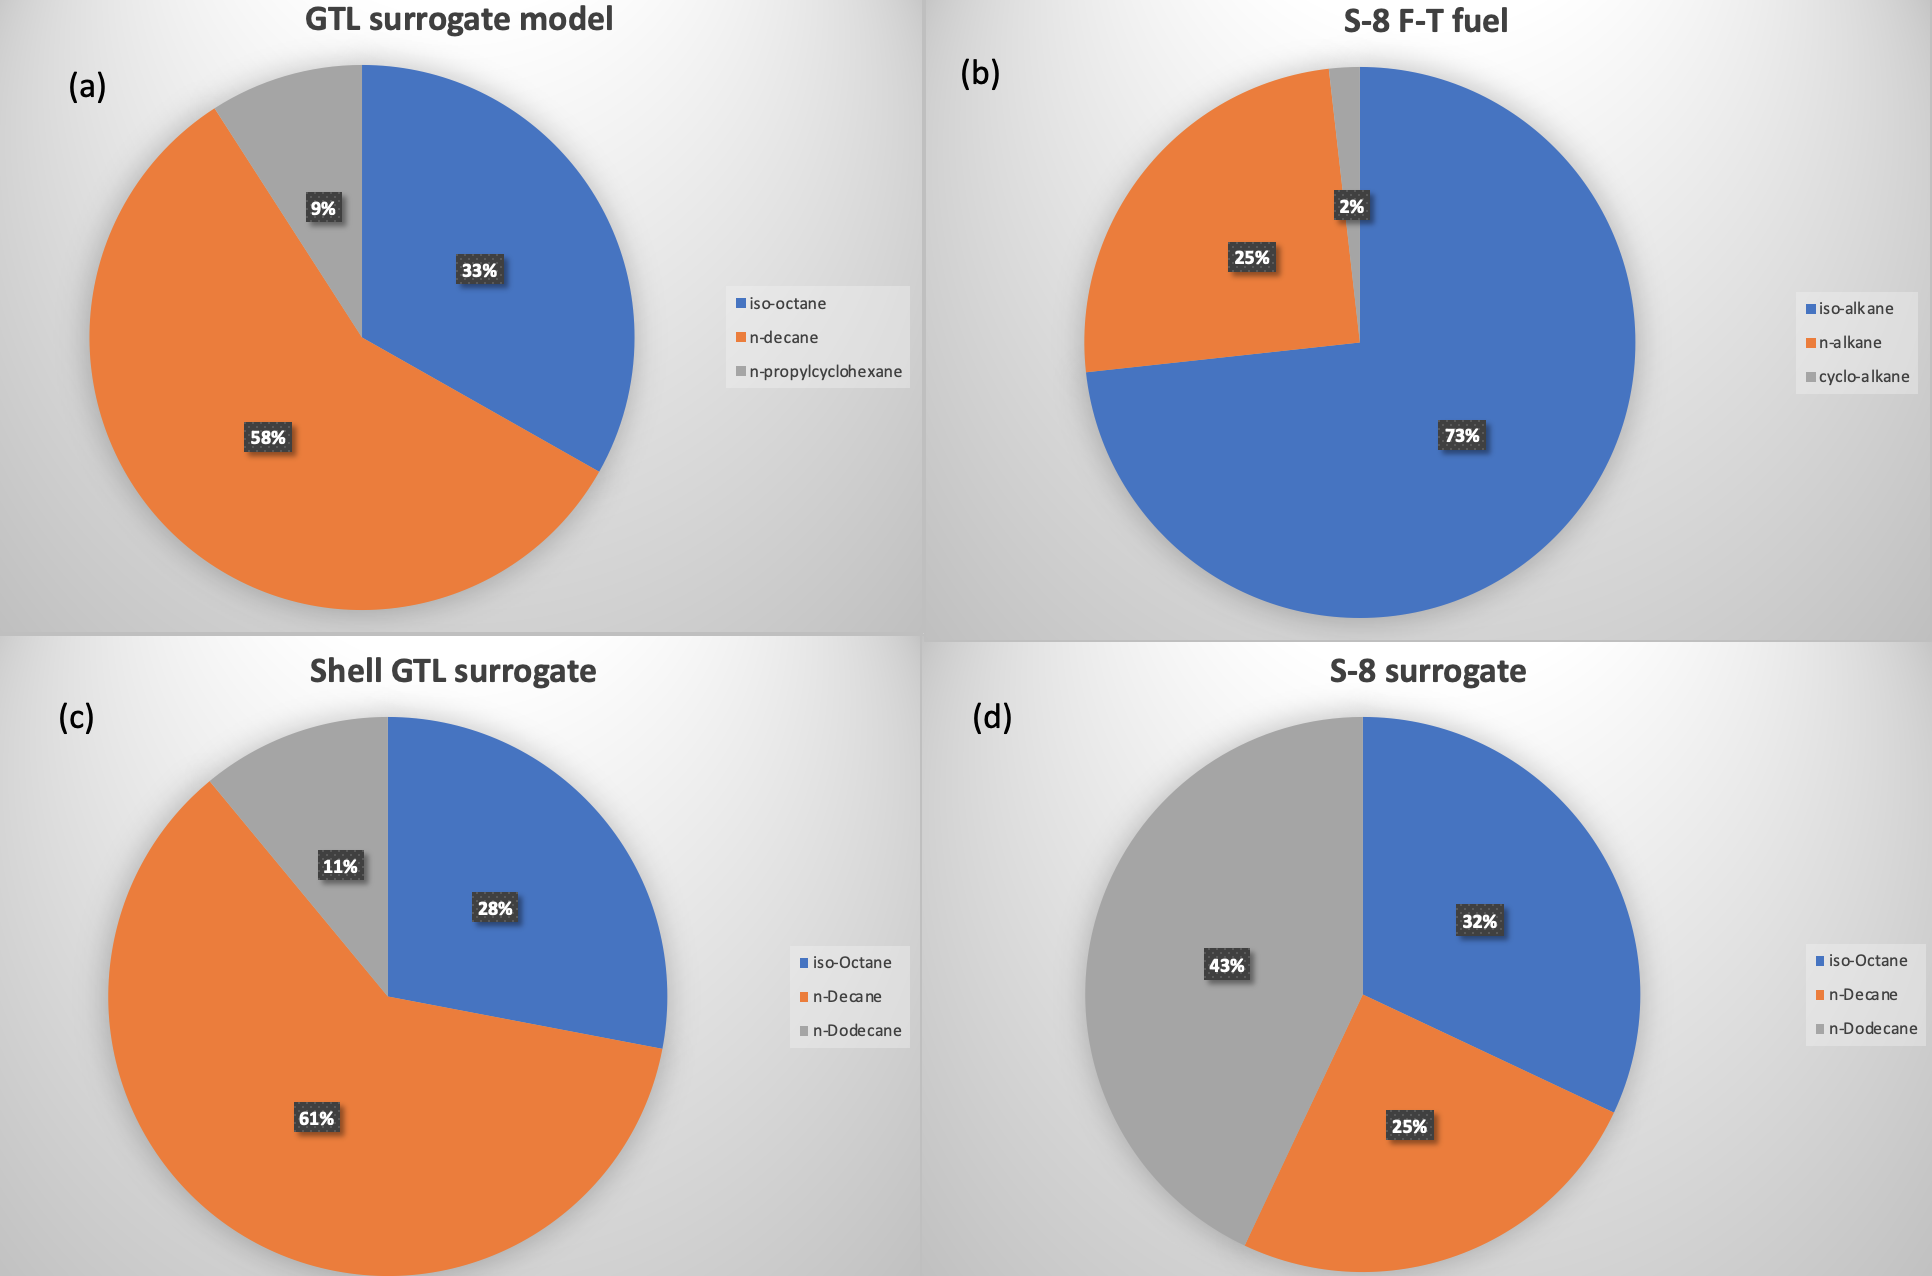
\includegraphics[width=\textwidth, height=\textheight, keepaspectratio]{images/GTL-composition.png}
    \caption{ (a) present work on GTL surrogate model blend \cite{Dagaut2014}, (b) S-8 F-T fuel in \% mol \cite{Naik2011DetailedFuels}, (c) Shell GTL surrogate fuel from Naik et al \cite{Naik2011DetailedFuels}, (d)S-8 surrogate fuel \cite{Moses2008COMPARATIVEREPORT}}
    \label{fig:GTL-composition}
\end{figure}


These methods are based on the mass spectrometry and chromatography analyses of a surrogate composition for primary reference fuel compounds. These surrogates are then used as the guideline to generate chemical kinetic model surrogate fuels that attempt to accurately represent the real fuels under engine-like conditions. The most commonly used blends usually contain paraffins (n-alkanes), olefins, iso-alkanes, naphthenes (cyclic alkanes) and aromatics (arenes). Aromatics are seldom added since it is well known as the primary species responsible for soot formation \cite{RoleOSTI.GOV}. The surrogate models are carefully chosen so they match both the chemical and physical properties like density, viscosity, specific weight, melting and boiling points, flash-points and auto-ignition temperatures. Similarly, the chemical properties such as ignition delay time of the fuel, concentration profiles of species in flow reactors and burning speed are usually the main properties that model generators try to match with the real fuel.

\section{Objective}
Now up until recently, according to the author's knowledge, from literature searches and researchers who have come up with surrogate mixture blends for GTLs, the best practice or framework to building GTL surrogate fuel blended models has been proposed; by either concatenation of the detailed chemical kinetic models of the pure primary reference fuels (PRFs) as given from the spectrometry analysis or a blended mixture of individual species from the onset of the model building process. These two approaches have not yet been tested to see if significant differences exist in the number of species and reactions generated when either of these approaches is used and which approach will closely match both the physical and chemical properties of these fuels as determined through experiments. 

This work focuses solely on the these two aforementioned steps for the automated generation of GTL surrogate fuel chemical kinetic model and its validation with experiments for congruence as well as the effects of each approach on the auto-ignition characteristics of these chemical kinetic blended models. These surrogate models are done with the intention on the best practice for computational modeling as well as completeness to the real surrogate fuel blends that engine designers can utilize in CFD simulations for further design analysis of combustor, fuel injector and other relevant design parameters during the development of new engines that utilize sustainable alternative jet and diesel fuels. 

This thesis is divided into six chapters with the second chapter focused on chemical kinetic mechanisms and the use of RMG in developing a detailed mechanism as well as its algorithm in mechanism generation and thermo-kinetic parameter estimation. The subsequent three separate chapters focus on the detailed kinetic model generation of the PRFs of n-decane, iso-octane and n-propyl-cyclohexane as well as their respective model validation in shock tubes for ignition delay times. The penultimate chapter is focused on the concatenation of the three PRF blends as well as the direct mechanism generation of the GTL fuel surrogate model with its mechanism validation in a shock tube for ignition delay time predictions. 
